\section{$\mathbf{A} = \mathbf{U\Sigma V}^{\dagger}$ Singular Value Decomposition}
\label{sec:svd}

The Singular Value Decomposition (SVD) exists for \underline{any} matrix $\mathbf{A}\in\mathbb{C}^{m\times n}$, and is a closely related alternative to the eigendecomposition (cf. section \ref{sec:diagonalization}) that works for non-square matrices. The contrast to diagonalization is that the eigenvectors and eigenvalues of $\mathbf{A}^{\dagger}\mathbf{A}$ and $\mathbf{A}\mathbf{A}^{\dagger}$ found, rather than to look for the eigensystem of $\mathbf{A}$ itself. The advantage is that $\mathbf{A}^{\dagger}\mathbf{A}$ and $\mathbf{A}\mathbf{A}^{\dagger}$ always have the convenient properties of being square, hermitian and positive semidefinite. 

SVD comes up incessantly in the context of data analysis. In general, the decomposition has the form:

\begin{equation}
\mathbf{A} = \mathbf{U\Sigma V^{\dagger}}
\end{equation}

Where $\mathbf{U}$ and $\mathbf{V}$ are unitary, and $\Sigma$ is a diagonal matrix with real and positive entries $\sigma_i^2$ along the diagonal, so that $\sigma_1 \geq \sigma^2_2 \geq ...\geq \sigma^2_n$. $\mathbf{U}$ is the matrix of left singular vectors, which are the eigenvectors of $\mathbf{A A^{\dagger}}$. $\mathbf{V}$ is the matrix of right singular vectors, which are the eigenvectors of $\mathbf{A^{\dagger} A}$. The singular values are the square roots of the eigenvalues of $\mathbf{A^{\dagger}A}$ or, equivalently, $\mathbf{AA^{\dagger}}$. If the $\mathbf{A}$ happens to be square and symmetric ($\mathbf{A}=\mathbf{A^T}$, cf. section \ref{sec:hermitian}), then the singular values are simply the absolute values of the eigenvalues of $\mathbf{A}$. The right and left singular vectors of the matrix are orthonormal bases that respectively span the column and row space of $\mathbf{A}$. The number of singular values of $\mathbf{A}$ is the rank of $\mathbf{A}$.
\\
The singular values are always real and positive or zero, because $\mathbf{A^{\dagger} A}$ and $\mathbf{A A^{\dagger}}$ are  hermitian and positive semidefinite (cf. sections \ref{sec:hermitian}, \ref{sec:definite}). When the matrix $\mathbf{A}$ has purely real entries, then the left and right singular vectors are also real, which is not necessarily the case for complex $\mathbf{A}$.
\\

The SVD of a matrix is unique up to the sign columns in $\mathbf{U}$ and $\mathbf{V}$. That is, the SVD is valid under transforming $\mathbf{u}_i, \mathbf{v}_i \rightarrow -\mathbf{u}_i, -\mathbf{v}_i $ if $\mathbf{u}_i$ and $ \mathbf{v}_i$ are the $i$th vectors in $\mathbf{U}$ and $\mathbf{V}$. This has the consequence that the basis of singular vectors that is found using SVD does not remain consistently oriented in the presence or noise or the slow evolution of a system. This is addressed in greater length in section \ref{sec:datasvd} on performing SVD specifically on data matrices.

\subsection{Full and Economy SVDs}
While these properties are always true, unfortunately people use a range of conventions when it comes to the size of $\mathbf{U}$, $\mathbf{\Sigma}$ and $\mathbf{V}$. \\

The first convention is for $\mathbf{U}$ and $\mathbf{V}$ to be square, in which case they contain the full set of left and right singular vectors, and $\Sigma$ has dimension $m\times n$, with $0$ entries in rows $i>n$. This is known as the \textit{full SVD}.\\

\citeasnoun{friedman2001elements} uses the the convention where $\Sigma$ is square, i.e. $\mathbf{U}:\ m\times n$, $\mathbf{\Sigma}:\ n\times n$ and $\mathbf{V}:\ n\times n$. This means that $U$ does not contain the full set of $m$ left singular vectors. Note that, in this case, $\mathbf{U^{\dagger}}\mathbf{U} = \mathbf{I}$ but $\mathbf{U}\mathbf{U^{\dagger}} \neq \mathbf{I}$. \possessivecite{friedman2001elements} convention is of advantage in the context of data analysis, where the data matrix tends to be "tall and skinny" (i.e. $m>>n$), and only the first $n$ left singular vectors are relevant. Also, a letting $\Sigma$ be a square matrix significantly simplifies calculations. \possessivecite{friedman2001elements} is known as the \textit{economy} or \textit{compact} SVD.\\

The two different layouts are illustrated in Figure \ref{fig:full_vs_economy_svd}, which I brazenly copied from \citeasnoun{mathworkseigs}.

\begin{figure}
\centering
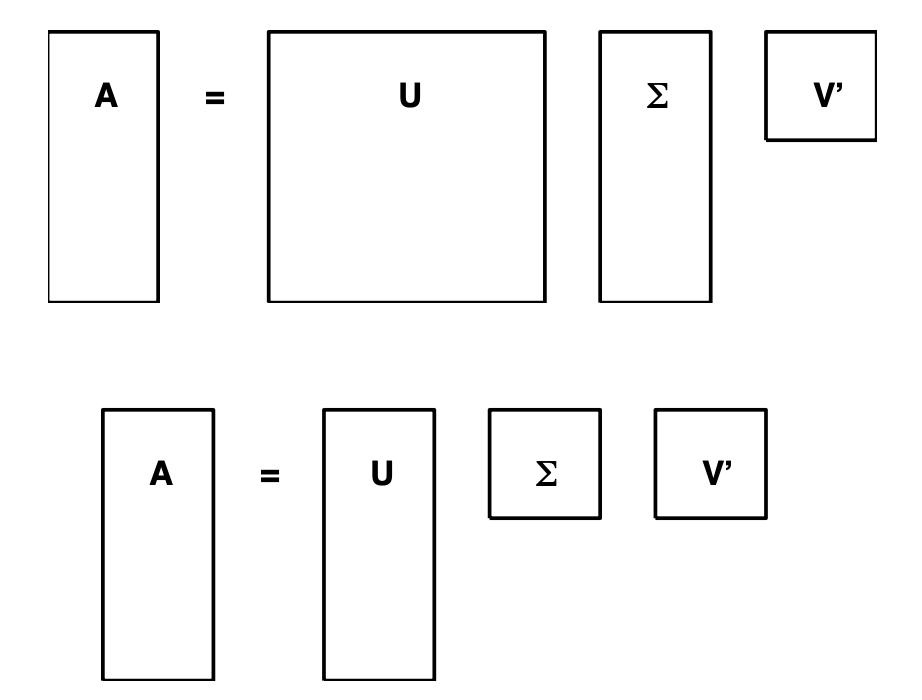
\includegraphics[scale=0.5]{full_vs_economy_svd.png}
\caption{Dimensions for Full vs. Economy SVDs}
\label{fig:full_vs_economy_svd}
\end{figure}

\subsection{Matrix Approximation}
The SVD enables the decomposition of the matrix into a sum:

\begin{equation}
\mathbf{A} = \sum_{i=1}^n \sigma_i (\mathbf{u}_i \otimes \mathbf{v}_i)
\end{equation}

Which may be truncated at some rank $r$, resulting in a rank-$r$ approximation to $\mathbf{A}$. This is known as the \textit{truncated singular value estimator} (TSVD):

\begin{equation}
\mathbf{\hat{A}} = \sum_{i=1}^r \sigma_i (\mathbf{u}_i \otimes \mathbf{v}_i)
\end{equation}

Where $\mathbf{u}_i$ is the $i$th left singular vector and $\mathbf{v}_i$ is the $i$th right singular vector. Following the Eckart-Young-Mirsky Theorem, taking the first $r \leq n$ terms of this series is the best rank-$r$ approximation to $\mathbf{A}$ under the Frobenius norm of the error, i.e.  $\underset{\mathrm{rank}(\mathbf{A}^{(r)})=r\leq n}{\argmin} ||\mathbf{A^r}-\mathbf{A}||_F$. The Frobenius norm essentially measures the elementwise mean squares error (MSE), cf. section \ref{sec:frobenius}).\\

In the context of data analysis, the reduced rank representation of a data matrix $\mathbf{A}$ acts as a filter in which the components that explain less of the variance in the dataset are removed, with the hope being that these correspond to noise. The intuition is that noise probably originates from a random process, so that components that correspond to noise have weak correlation with the entries of the dataset and therefore small singular values. On the other hand, the signal probably systematic, so that the components that correspond to the signal have larger singular value. Since TSVD minimizes the average mean squares error (AMSE) amounts to the rank-$r$ maximum likelihood estimator of the signal under the assumption of normally distributed noise with mean zero. 

By virtue of being expressible in terms of fewer base vectors, a lower rank approximation is also a very effective compression method. For a more elaborate discussion of SVD in data analysis, see section \ref{sec:datasvd}. In a practical context, the question of selecting the appropriate rank of the approximation emerges. Section \ref{sec:svd_truncation} covers a few approaches to this.


% Geometric interpretation
\subsection{Geometric Interpretation of SVD}
A common intuitive interpretation of $\mathbf{U}$, $\mathbf{\Sigma}$ and $\mathbf{V}$ is to see them as a decomposition of the action of the matrix $\mathbf{A}\in\mathbb{R}^{m\times n}$ into a rotation, a stretching and another rotation. Let $\{\mathbf{x} : |\mathbf{x}|=1 \}$ be the points on the surface of a unit sphere, then $\mathbf{Ax}$:

\begin{itemize}
\item $\mathbf{V}$ rotates the unit sphere, which has no effect. However, it expresses each $\mathbf{x}$ in terms of a different coordinate system (the right singular basis of $\mathbf{A}$). 
\item $\mathbf{\Sigma}$ stretches the unit sphere into an ellipse with principal axes aligned to that coordinate system.
\item $\mathbf{U}$ rotates the ellipse.
\end{itemize}

In the above, "rotation" might include coordinate flips that are undone by $\mathbf{U}$ following $\mathbf{V}$. Alternatively, for a vector $\mathbf{v}\in\mathbf{R}^{n}$, the operation $\mathbf{Av}$:

\begin{itemize}
\item $\mathbf{V}$ is a change of basis matrix that expresses $\mathbf{x}$ in terms of a right eigenbasis of $\mathbf{A}$
\item $\mathbf{\Sigma}$ performs a stretching in that basis
\item $\mathbf{U}$ is a change of basis from the right eigenspace into the left eigenspace of $\mathbf{A}$. 
\end{itemize}

